% !TeX spellcheck = en_US
\documentclass[12pt]{report}
\usepackage[a4paper, total={7in, 9in}]{geometry}
\usepackage{setspace} %Line spacing
\onehalfspacing

\usepackage{pdfpages}

\usepackage{fancyhdr}
\usepackage{lastpage}

% For the chapters not to modify the page style
\usepackage{titlesec}
\titleformat{\chapter}{\bfseries}{\huge\arabic{chapter}.}{10pt}{\huge}
\titleclass{\chapter}{straight}

%REFERENCES
\usepackage{siunitx, multirow, booktabs}
\usepackage{blindtext,alltt}
\usepackage[backend=bibtex, style=numeric, sorting=none, locallabelwidth]{biblatex}
\addbibresource{/home/leonidas/Documents/References.bib}

\usepackage{listings}

\usepackage{wrapfig}
\usepackage{array}
\usepackage{multicol}
\usepackage{url}
\usepackage[nottoc]{tocbibind} %Add references to index.
\usepackage{amsmath, amssymb}
\usepackage{upgreek, dsfont, mathrsfs}
\usepackage{stmaryrd}


\usepackage[breakable]{tcolorbox}
\usepackage{parskip} % Stop auto-indenting (to mimic markdown behaviour)


% Basic figure setup, for now with no caption control since it's done
% automatically by Pandoc (which extracts ![](path) syntax from Markdown).
\usepackage{graphicx}
\usepackage{caption}

%Footnoe symbol instead of numbers
%1   asterisk        *   2   dagger      †   3   double dagger       ‡
%4   section symbol  §   5   paragraph   ¶   6   parallel lines      ‖
%7   two asterisks   **  8   two daggers ††  9   two double daggers  ‡‡
\usepackage[symbol]{footmisc}
\renewcommand{\thefootnote}{\fnsymbol{footnote}}

\usepackage{float}
\floatplacement{figure}{H} % forces figures to be placed at the correct location

\usepackage{xcolor} % Allow colors to be defined
\usepackage{enumerate} % Needed for markdown enumerations to work
\usepackage{geometry} % Used to adjust the document margins
\usepackage{amsmath} % Equations
\usepackage{amssymb} % Equations
\usepackage{textcomp} % defines textquotesingle
% Hack from http://tex.stackexchange.com/a/47451/13684:
\AtBeginDocument{%
	\def\PYZsq{\textquotesingle}% Upright quotes in Pygmentized code
}
\usepackage{upquote} % Upright quotes for verbatim code
\usepackage{eurosym} % defines \euro

\usepackage{iftex}
\ifPDFTeX
\IfFileExists{alphabeta.sty}{
	\usepackage{alphabeta}
}{
	\usepackage[mathletters]{ucs}
	\usepackage[utf8x]{inputenc}
}
\else
\usepackage{fontspec}
\usepackage{unicode-math}
\fi


% The hyperref package gives us a pdf with properly built
% internal navigation ('pdf bookmarks' for the table of contents,
% internal cross-reference links, web links for URLs, etc.)
\usepackage{hyperref}
% The default LaTeX title has an obnoxious amount of whitespace. By default,
% titling removes some of it. It also provides customization options.
\usepackage{titling}
\usepackage{longtable} % longtable support required by pandoc >1.10
\usepackage{booktabs}  % table support for pandoc > 1.12.2
\usepackage{array}     % table support for pandoc >= 2.11.3
\usepackage{calc}      % table minipage width calculation for pandoc >= 2.11.1
\usepackage[inline]{enumitem} % IRkernel/repr support (it uses the enumerate* environment)
\usepackage[normalem]{ulem} % ulem is needed to support strikethroughs (\sout)
% normalem makes italics be italics, not underlines
\usepackage{mathrsfs}



% Colors for the hyperref package
\definecolor{urlcolor}{rgb}{0,.145,.698}
\definecolor{linkcolor}{rgb}{.71,0.21,0.01}
\definecolor{citecolor}{rgb}{.12,.54,.11}

% ANSI colors
\definecolor{ansi-black}{HTML}{3E424D}
\definecolor{ansi-black-intense}{HTML}{282C36}
\definecolor{ansi-red}{HTML}{E75C58}
\definecolor{ansi-red-intense}{HTML}{B22B31}
\definecolor{ansi-green}{HTML}{00A250}
\definecolor{ansi-green-intense}{HTML}{007427}
\definecolor{ansi-yellow}{HTML}{DDB62B}
\definecolor{ansi-yellow-intense}{HTML}{B27D12}
\definecolor{ansi-blue}{HTML}{208FFB}
\definecolor{ansi-blue-intense}{HTML}{0065CA}
\definecolor{ansi-magenta}{HTML}{D160C4}
\definecolor{ansi-magenta-intense}{HTML}{A03196}
\definecolor{ansi-cyan}{HTML}{60C6C8}
\definecolor{ansi-cyan-intense}{HTML}{258F8F}
\definecolor{ansi-white}{HTML}{C5C1B4}
\definecolor{ansi-white-intense}{HTML}{A1A6B2}
\definecolor{ansi-default-inverse-fg}{HTML}{FFFFFF}
\definecolor{ansi-default-inverse-bg}{HTML}{000000}

% common color for the border for error outputs.
\definecolor{outerrorbackground}{HTML}{FFDFDF}

% Prevent overflowing lines due to hard-to-break entities
\sloppy 
% Setup hyperref package
\hypersetup{
	breaklinks=true,  % so long urls are correctly broken across lines
	colorlinks=true,
	urlcolor=urlcolor,
	linkcolor=linkcolor,
	citecolor=citecolor,
}

\definecolor{codegreen}{rgb}{0,0.6,0}
\definecolor{codegray}{rgb}{0.5,0.5,0.5}
\definecolor{codepurple}{rgb}{0.58,0,0.82}
\definecolor{backcolour}{rgb}{0.95,0.95,0.92}

\lstdefinestyle{mystyle}{
	backgroundcolor=\color{backcolour},   
	commentstyle=\color{codegreen},
	keywordstyle=\color{magenta},
	numberstyle=\tiny\color{codegray},
	stringstyle=\color{codepurple},
	basicstyle=\ttfamily\footnotesize,
	breakatwhitespace=false,         
	breaklines=true,                 
	captionpos=b,                    
	keepspaces=true,                 
	numbers=left,                    
	numbersep=5pt,                  
	showspaces=false,                
	showstringspaces=false,
	showtabs=false,                  
	tabsize=2
}

\lstset{style=mystyle}

\pagestyle{fancy}
\fancyhf{}
\rhead{}
\lhead{THESIS PROJECT $|$ \textcolor{red}{MONITORED HIVES FOR HONEYBEES}}
\lfoot{Universidad Autónoma de Chihuahua}
\rfoot{Page \thepage \hspace{1pt} of \pageref{LastPage}}

\renewcommand{\headrulewidth}{0.5pt} %ancho de la recta del encabezado superior


\begin{document}
	
	%\thispagestyle{empty}
	\begin{titlepage}
		\begin{center}
			\begin{tabular}{c}
				
\includegraphics[scale=0.2]{BN_uach.png}\\[3.5ex]
				\textbf{\LARGE Universidad Autónoma de Chihuahua}\\[3.5ex]
				\textbf{\Large Facultad de Ingeniería}\\[3.5ex]
				\hline\\[3ex]
				\begin{minipage}{17cm}
					\centering
					\begin{doublespace}
						\textbf{\LARGE MONITORED HIVES FOR HONEYBEES: Implementing a Microphone on the Monitoring Device}
					\end{doublespace}
				\end{minipage}\\[3.5ex]
				\hline
			\end{tabular}\vfill
			{\large Thesis Protocol.}\\\vfill
			{\large \textbf{Student:} Leonardo Rafael León Mora.}\\\vfill
			{\large \textbf{Thesis director:} Dr. Daniel Espinobarro Velázquez.}\\\vfill
			{\large \textbf{Suggested advisors:}}\\[3.5ex]
			\begin{itemize}
				\item {\large M.C. Carlos Hugo Larrinúa Pacheco.}\\[3.5ex]
				\item {\large M.I. Joseph Isaac Ramírez Hernández.}\\[3.5ex]
			\end{itemize}
			\vfill
			{\large \textbf{Chihuahua, Chih.,} \today.}\\[3.5ex]
		\end{center}
	\end{titlepage}
	
	
	%------------------------------------------------------------------------------------------
	% 1. Dynamic Noise Filtering for Multi-Class Classification of Beehive Audio Data.
	%------------------------------------------------------------------------------------------
	
	\chapter{READINGS}
	
	Cada vez que se revisa la colmena de forma manual existe la posiblidad de matar a la reina al extraer uno de los bastidores de la colmena, lo que puede llevar a la perdida total de la misma.
	
	\chapter{Dániel Tamás Várkonyi, José Luis Seixas Junior, Tomáš Horváth.}
	
	\section{Introduction}
	
	In the majority of apiaries, identification of the health condition of a bee colony is done manually by opening and inspecting the hive. Opening the hive, however, introduces certain stress to the colony while changing the micro-climate within the hive. Afterward, bees have to expend considerable energy to re-establish the equilibrium within the beehive. Consequently, \textbf{frequent manual inspection of a hive reduces the amount of honey the given bee colony produces}.
	
	\par Analyzing the colony's sound might reveal certain anomalous events within the hive, like the presence of an intruder or \textbf{the preparation of the colony for swarming}. The first technological approaches used for monitoring bees' condition via audio analysis were conducted in the late 20th century using spectral analysis in the range of $0-3$ kHz \cite{dietlein1985spectral_analysis}.
	
	\par Applying machine learning ({\tt ML}) to audio analysis for bee queen presence detection and swarming prediction leads to a basic binary classification task, i. e. predicting if the queen is present or not and if the colony is swarming or not. Moreover, \textbf{the sound of a bee colony in a ``queenless'' or swarming state is well distinguishable from its sounds when a queen is present or the colony is not swarming} \cite{allen1956behaviourbeeswarming, hord2013behavioraudioanalysis}. \textbf{The stress level of the colony exposed to an ``anomaly'' likely implies a substantially different sound from the one when being in a normal state}.\\
	An important issue, contravening the approaches found in the literature, is that \textbf{these problems might not necessarily correspond to binary classification tasks}. For example, identification of various (more than two) types of diseases, intrusion detection by different pests, or estimation of exposure of bees to diverse palettes of chemicals, naturally, calls for multi-label or even multi-class approaches. An assumption here, posing possible difficulties for application of ML techniques, is that \textbf{bee sounds corresponding to various classes (labels) might not be so easily distinguishable from each other} as they usually are in the before mentioned binary cases where ``anomalous'' and ``normal'' states are well-detectable even for humans.
	
	\begin{figure}
		\centering
		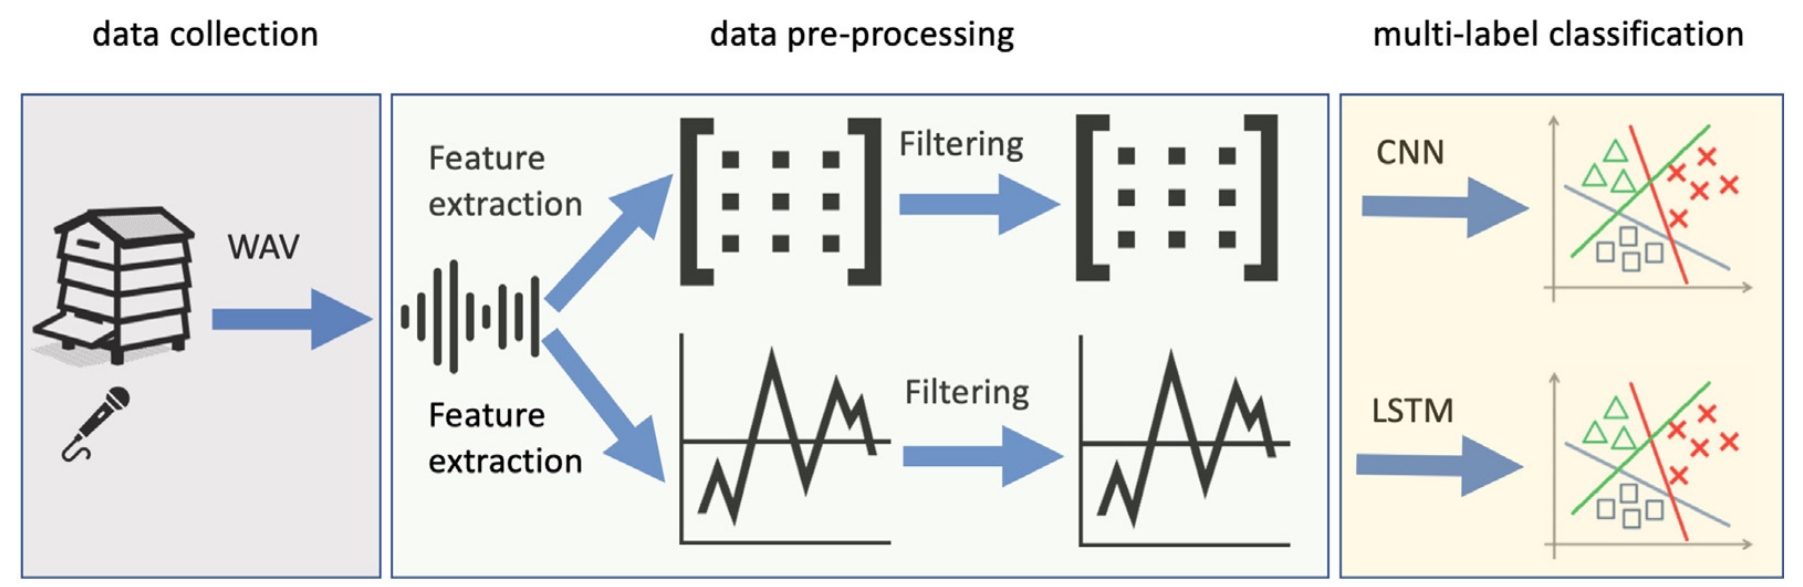
\includegraphics[scale = 0.25]{beeaudioworkflow.png}
		\caption{A general audio data analytics workflow used in our experiments.}
		\label{fig:audioworkflow}
	\end{figure}
	
	\par There is a huge gap int he literature considering multi-label or multi-class classification of bee audio data. According to our knowledge. The only work related to multi-label bee sound classification \cite{gradivsek2017predictingbumblebees}, is focused on identifying 12 bumblebee species from their buzzing sounds (from a small-scale dataset using traditional {\tt ML} techniques, such that naïve Bayes decision trees, support vector machines, and random forests).
	
	\begin{itemize}
		\item \textbf{Problem \# 1}. The classification accuracy of the audio data analytics work flow, shown in figure \ref{fig:audioworkflow}, does not only depend on the discriminative power of the used {\tt ML} techniques, but also, on the used pre-processing steps. One of the basics problems of audio signals is that, even after filtering out irrelevant information, the resulting data represented as time-series have very high dimensionality. Feature extraction ({\tt FE}) methods are utilized to extract and represent the most important features within the audio signal in a compact form (time-series or spectrograms), preserving a significant portion of its original information content. After {\tt FE}, {\tt ML} techniques can be applied on the data (depending on the amount, dimensionality and the task intended to be solved).
		
		\item \textbf{Problem \# 2}. According to our knowledge, there is no reference in the literature to a survey comparing various combinations of audio {\tt FE} (image or time-series), noise filtering ({\tt NF}) and {\tt ML} (image or time-series classification) techniques for bee sound analytics. including thorough hyper-parameter ({\tt HP}) tuning and validation procedures as well as utilizing large datasets.
		
		\item \textbf{Problem \# 3}. According to our knowledge, there is no large-scale publicly available bee sound benchmark data suitable for research on multi-label or multi-class bee sound classification approaches.\\
		Several {\tt ML} developments, e.g. various deep learning ({\tt DL}) models, have been developed working efficiently on specific problems related to audio processing like, for example, human speech recognition. However, our experiments showed that \textbf{these methods are not performing well in case of a multi-label bee sound classification problem} in which the difference between various classes is inconspicuous.
		
		\item \textbf{Problem \# 4}. The main reason for the poor performance of state-of-the-art {\tt ML} models for multi-label bee sound classification lies in the poor performance of the used {\tt NF} methods, which seems to be not suitable for bee sound data.
	\end{itemize}
	
	\section{Beehive Sound Analytics}
	
	In the explained experiments of this paper, despite the suggested frequency range of 0-4 kHz by Hord and Shook (2013) and Qandour et al. (2014), for	the sake of investigation, the frequency range of 0-8 KHz has been	considered. Thus, before the {\tt FE} step, frequencies beyond this range are filtered out.
	
	\subsection{\textit{Audio feature extraction} ({\tt FE})}
	
	The input of {\tt FE} is an audio file in the form of a real-valued time-series data
	\begin{equation*}
		x(t) = \{ x_t \; | \; 0 \le t < N \} = \{ x_0 \, , \; x_1 \, , \; ... \, , \; x_{N - 1} \} \; ,
	\end{equation*}
	
	of length $N$, where $x$ represents the amplitude of the signal in time $t$.\\
	
	The goal of {\tt FE} is to transform or represent $x(t)$ via features carrying important information (preferably, the whole time interval of the recording).
	
	\begin{itemize}
		\item \textbf{\textit{Short-Time Fourier Transform} ({\tt STFT})}
		\par Discrete-Time Fourier Transformation ({\tt DTFT}) transforms $x_n$ into another complex series $y(k) = \{ y_k \; | \; 1 \le k \le K \} = \{ y_1 \, , \; y_2 \, , \; ... \, , \; y_k \}$
		\begin{equation}\label{eq:1}
			y_k = \sum_{n = 0}^{N - 1} x_n \cdot e^{-i \, \frac{2 \pi}{N}kn} = \sum_{n = 0}^{N-1} x_n \left[ \cos{\left( \frac{2 \pi}{N} kn \right)} - i \cdot \sin{\left( \frac{2 \pi}{N} kn \right)} \right] \; ,
		\end{equation}
		which represents the audio data $x(n)$ in the frequency domain instead of the time domain. In case of {\tt STFT}, $x(n)$ is broken into windows $w(n - m)$ with a window size $m$, which might overlap. {\tt DTFT} is applied to each window, recording the magnitude (and phase) of $x(n)$ for each frequency and time. {\tt STFT} can be expressed as {\tt DTFT} on $x(n)w(n - m)$, such that
		\begin{equation}\label{eq:2}
			y_k = \sum_{n = 0}^{N - 1} x_n w(n - m) \cdot e^{-i \, \frac{2 \pi}{N} kn} \; .
		\end{equation}
		The information of the signal's magnitude can be represented in a 2D ``time-frequency'' matrix called \textbf{spectrogram}.
		
		\item \textbf{\textit{Chroma}}
		\par Chroma features represent he tonal content of an audio signal $x(n)$. The extraction process includes the following steps:
		\begin{enumerate}
			\item Providing {\tt STFT} for frequency analysis.
			\item Filtering frequency.
			\item Peak detection.
			\item Reference frequency computation.
			\item Pitch class mapping.
			\item Normalizing the feature.
		\end{enumerate}
	
		\item \textbf{\textit{Mel-frequency Cepstral coefficients} ({\tt MFCC})}.
		\par Extracting {\tt MFCC} starts by computing {\tt DTFT} of the signal $x(n)$, resulting in $y(k)$, as introduce in Eq.(\ref{eq:1}). Then the Mel spectrum of the magnitude spectrum is computed as
		\begin{equation}\label{eq:3}
% I do not know if the paper was right in here but I think it might be "M - 1" as the top of the sum
			s(m) = \sum_{n = 0}^{N - 1} \left[ {|y(k) |}^2 h_m(k) \right] \; ; \quad 0 \le m \le M - 1 \; ,
		\end{equation}
		where $M$ is the total number of triangular Mel weighting filters and $h_m(k)$ is the weight given to the $k$th energy spectrum bin, contributing to the $m$th output band, expressed as
		\begin{align*}
			h_m(k) =
			\begin{cases}
				\frac{2 (k - f (m - 1))}{f(m) - f(m - 1)} \; , &\text{ if } f(m - 1) \le k < f(m) \; , \\
				\frac{2(f (m + 1) - k)}{f(m + 1) - f(m)} \; , &\text{ if } f(m) \le k < f(m + 1) \; , \\
				0 \; , &\text{ otherwise.}
			\end{cases}
		\end{align*}
		Finally, Discrete Cosine Transformation is applied such as
		\begin{equation*}
			c(n) = \sum_{n = 0}^{M - 1} \log{(s(m))} \cdot \cos{\left( \frac{\pi n (m - 0.5)}{M} \right)} \; , \text{ where } 0 \le n \le C - 1 \; ,
		\end{equation*}
		$c(n)$ are the Cepstral coefficients and $C$ is the number of {\tt MFCC}s.
		
		\item \textbf{{\tt MFCC} \textit{differential coefficients} ({\tt MFCC} delta)}
		\par The first order derivative of {\tt MFCC} (differential) coefficients are defined as
		\begin{equation}\label{eq:4}
			d_t = \frac{\sum_{n = 1}^{N} n \left( c_{t + n} - c_{t - n} \right)}{2 \sum_{n = 1}^{N} n^2} \; ,
		\end{equation}
		where $d_t$ is the delta coefficient of the frame $t$ in terms of {\tt MFCC}s from $c_{t + n}$ to $c_{t - n}$.
		
		\item \textbf{\textit{Spectral centroid} ({\tt SC})}
		\par A measure is used to characterize the spectrum, is defined as
		\begin{equation}\label{eq:5}
			SC(n) = \frac{\sum_{m = 0}^{N - 1} m \cdot {|X[n, \, m]|}^2}{\sum_{m = 0}^{N - 1} {|X[n, \, m]|}^2} \; .
		\end{equation}
		{\tt SC} indicates the center of frequency (``gravity centrum'') of the $n$th frame.
		
		\item \textbf{\textit{Zero-crossing rate} ({\tt ZCR})}
		\par {\tt ZCR} indicates the number of sign changes in the $n$th frame, defined by
		\begin{equation}\label{eq:6}
			ZCR(n) = \frac{1}{2N} \sum_{m = 1}^{N} |sgn(x[n + m]) - sgn(x[n + m - 1])| \; .
		\end{equation}
		{\tt ZCR} can be interpreted as a measurement of noisiness. The higher the {\tt ZCR} in a frame, the noisier the signal.
		\par The {\tt SC} and {\tt ZCR} {\tt FE} result in a time-series type output, and not in a spectrogram as in case of the other {\tt FE} methods introduced above.
	\end{itemize}
	
	\subsection{Multi-label audio data classification using machine learning ({\tt ML})}
	
	Depending on which method is being used, {\tt FE} might result in two different types of output, time-series data or a spectrogram (2D feature matrix), which can be seen as an image.
	
	\begin{itemize}
		\item \textbf{\textit{Time-series classification}}.
		
		\item \textbf{\textit{Image classification}}.
		
		\item \textbf{\textit{Noise filtering} ({\tt NF})}.
		
		\item \textbf{\textit{Laplacian filter}}.
		
		\item \textbf{\textit{Gaussian filter}}.
		
		\item \textbf{\textit{Laplacian of Gaussian filter}}.
		
		\item \textbf{\textit{Median filter}}.
		
		\item \textbf{\textit{High pass filter}}.
	\end{itemize}
	
	%------------------------------------------------------------------------------------------
	% 2. On the Importance of the Sound Emitted by Honey Bee Hives.
	%------------------------------------------------------------------------------------------
	
	\chapter{Alessandro Terenzi, Stefania Cecchi, and Susanna Spinsante}
	
    \section{Introduction}
    
    Honey bees not only produce honey, beeswax, royal jelly, and propolis, but they are at the basis of the plants pollination, playing a key role in the proliferation of both spontaneous and cultivated flora.\\
    One of the most recent and dangerous syndromes affecting honey bee colonies is the Colony Collapse Disorder (CCD), which is characterized by a sudden disappearance of honey bees from the hive.
    
    \par Large bee mortality can result in a loss of pollination services with negative ecological and economic impacts that could significantly affect the maintenance of wild plant diversity, wider ecosystem stability and crop production. In this context, the necessity of a continuous and intensive monitoring of bee hives' status emerges clearly.
    
    \par In recent years, a great improvement has come from the integration of web technologies and smart sensors. But, despite this approaches having shown good results, they still require remarkable computational power, several different types of sensors, and sometimes they impose some modifications to the hive physical structure.
    
    \par Modalities of vibroacoustic signal production include gross body movements, wing movements, high-frequency muscle contractions without wing movements, and pressing the thorax against the substrates or with another bee. Vibroacoustic signals modulate behaviors that affect swarming, and the queen's behavior during swarming. The sound can be recorded by means of microphones or accelerometers placed in specific spots inside or outside the hives, and then it can be analyzed to detect the colony health status.
    
    \section{Literature Review}
	
	\par Aristotle in one of his writings observed that, when a swarming is imminent, a particular sound is produced continuously by the bees, several days before the swarming event. A century later, Francis Huber discovered that the first young queens born emit a sound called tooting, and that other young queens, who are still sitting in their cells, respond with another sound called quacking. In 1964, Wenner et al. \cite{wenner1964sound} performed one of the first spectral analyses on the honey bee's sound. They discovered that the waggle dance is used by bees to communicate within the colony the information about the distance and position of flowers. During the dance, \textbf{bees emit a specific pulsed sound, in which the number of pulses is proportional to the distance between the colony and the flowers}. Wenner also deepened the study about tooting, showing that this sound is composed of two different pulses, the first is a long pulse of $1s$ duration followed by shorter pulses, with a fundamental frequency of 500 Hz and some overtones. The quacking has a lower fundamental frequency and starts with shorter pulses.
	
	\par In 1985, Dietlein et al. \cite{dietlein1985spectral_analysis} performed a longer study acquiring and analyzing the sound from three different colonies for over a year, showing that there are some significant variations in the amplitude and frequencies of the sound produced in different seasons. Moreover, a frequency analysis has also shown that the spectral content of the signal changes with the seasons and the hour of the day. Then, in 1986, Michelsen et al. \cite{michelsen1986sound} performed a study more focused on the sound emitted during the waggle dance, analyzing both the vibration and the airborne sound produced. Since it is performed inside the hive in the dark, bees cannot rely on their sight to see the dance, and they must use other communication means, such as vibration, airborne sound, and chemical transmission. Michelsen discovered that no vibration is produced during the dance, and that all of the information is passed through the airborne sounds. The waggle sound is a pulsed sound, with 20 ms-long pulses at the frequency of 250-300 Hz.\\
	The second part of Michelsen's work is more focused on the mechanical aspects of the propagation of sound and vibration inside the colony. \textbf{Bees seem to freeze at specific frequencies}, and this led Michelsen to speculate that these particular signals are used by bees to quiet the colony, in order to allow a better transmission of important messages.
	
	\subsection{The 21st Century and the Technological Advancement}
	
	Within the last twenty years, technological progress has allowed the application of new solutions such as digital signal processing, ML, and low cost smart sensors, enabling new discoveries. Sound spectrograms have shown that there is a quick change in the frequency content during swarming. Before the swarming, most of the energy content of the signal is around 150 Hz, while, during swarming, it jumps to 500 Hz. Moreover, \textbf{the joint analysis of sound, temperature, and humidity} has shown that during swarming, \textbf{there is an increase in sound amplitude, and, meanwhile, temperature and humidity decrease}.
	
	%------------------------------------------------------------------------------------------
	% 3. Honeybees Swarming Detection Approach by Sound Signal Processing.
	%------------------------------------------------------------------------------------------
	
	\chapter{Aleksandra Zlatkova, Zivko Kokolanski and Dimitar Tashkovski}
	
	Swarming of honeybees is one of the biggest problems for the hobbyist-beekeepers.
	
	\section{Introduction}
	
	Honey bee or Apis mellifera is one of several types of bees, their role in pollination is estimated to be around 90\%. Bees are organized in colonies of 50,000 bees on average. The colony include queen bee, workers and drones. Once inside the hive, bees communicate through pheromones, sound and vibrations. Swarming is a natural process that means part of honeybees runaway from the beehive and stablish a new colony. 
	
	\par Usually, beekeepers are hobbyist whose hives are located in rural environments, long from their homes. \textit{They do not see the hive too often, and there is the possibility that swarming occurs between those days}. \textbf{This reason imposes the need of a monitoring system}. In the recent years, few studies related swarming with sound, temperature and humidity inside \textit{within the colony} and weight of the hive.
	
	\section{Method}
	
	The dataset contains audio samples recorded before and after swarming. Despite the processing, recordings were visual observed to verify if there are some disorders. For example, the bees become upset and change their behavior during every human activity in the beehive. Those audio files that had similar disorders were excluded from further analyses. Afterwards, data samples were normalized in range [-1, 1].
	
	\par The frequencies in a signal change over time, so in most cases it does not make sense to implement Fourier Transform across the entire signal.
	
	%------------------------------------------------------------------------------------------
	% 4. A Smart Sensor-Based Measurement System for Advanced Bee Hive Monitoring.
	%------------------------------------------------------------------------------------------
	
	\chapter{Stefania Cecchi, Susanna Spinsante, Alessandro Terenzi and Simone Orcioni}
	
	\section{Introduction}
	
	These industrious insects do not only produce honey, beeswax, royal jelly, and propolis, but they are at the basis of the plants' pollination process, playing a key role in the proliferation of both spontaneous and cultivated flora. For these reasons, it is of utmost importance to design solutions aimed at preserving and supporting the honey bees' healthy existence.\\
	Colony collapse disorder (CCD) is a recent, pervasive syndrome affecting honey bee colonies, which is characterized by a sudden disappearance of honey bees from the hive. CDD has emphasized the importance of enabling a continuous, multi-parametric, and extensive monitoring of the beehives, to investigate factors that may negatively affect the life cycle of bees. A continuous monitoring and an automatic analysis of the beehives' status can help to safeguard and to protect their life, by early detection of potential threats.
	
	\par There are several approaches focused in many areas with respect to the analysis of beehives like:
	\begin{itemize}
		\item General monitoring system. In particular, temperature, humidity, air quality sensors, and an \textbf{accelerometer} compass are installed within the hive.
		\item Adoption of wireless technologies. Another way to apply the monitoring of the hive is by creating a wireless sensor network system to check the hive status far from the place where it is placed.
		\item Systems exploiting computer vision-based approaches. To analyze the behavior of honey bees and their flight activities outside the hive.
	\end{itemize}
	
	Starting from the state of art related to monitoring systems and technological developments, this work aims at developing a complete, multi-parametric smart sensor-based measurement system capable of monitoring in real-time a colony of beehives, and discriminating several events, such as swarming event, beehive theft, honey gathering, reserve food lack, decrease of bees' number due to illness.
	
	\section{State of Art of Measurement Systems for Beehives}
	
	\subsection{Sound measurement}
	
	The sound analysis of the beehives is a useful technique applied to determine the bees' state in a noninvasive manner.
	
	\par The bees communicate each other using vibration and sound signals such as gross body movements, wing movements, high-frequency muscle contractions without wing movements, and pressing the thorax against the substrates or another bee. These signals are also strictly related to particular events, such as swarming and queen behavior during swarming as we will see in what follows.
	
	\par As an alternative to the use of microphones, accelerometers sensors could also be used to sample the hive vibrations. The sound have been analyzed in the frequency domain by means of the Fourier transform before and after the swarming event and changes in terms of frequencies and amplitudes have been found. During the swarming event, it is also possible to retrieve from the audio analysis the presence of the queen bee. As a matter of fact, young queens emit piping sounds during the swarming process. These sounds can be identified through a frequency analysis and since they are characterized by a specific frequency, the allows to detect the presence of young queen inside the hive. Moreover, during the year, also the worker bees produce different piping sounds with relation to the presence or absence of the queen in the colony.
	
	\par The use of microphones or accelerometers allows getting more detailed information on the general state of the hive.
	
	\subsubsection{Presence of Airborne Toxics in the Hive}
	
	This system is based on a profiling of the acoustic signatures of free-flying honey bee colonies, analyzing the resulting acoustic sounds to identify anomalies with relation to the specific properties of those acoustic sounds.
	
	\par Recently, the use of Deep Learning and Machine Learning has been introduced to classify the recorded audio samples and to define an objective status of the analyzed beehives.
	
	%------------------------------------------------------------------------------------------
	% 5. Processing of Multi-Modal Environmental Signals Recorded from a ‘Smart’ Beehive.
	%------------------------------------------------------------------------------------------
	
	\chapter{Gordon Hunter, Donald Howard, Sylvain Gauvreau, Olga Duran, Rosa Busquets}
	
	\section{Introduction}
	
	The population of bees has experienced a marked decline in many countries, which is likely to have very serious consequences for agriculture and other plant life.
	
	
	
	%------------------------------------------------------------------------------------------
	% 6. METODOLOGÍA.
	%------------------------------------------------------------------------------------------
	
	\chapter{METODOLOGÍA}
	
	
	%------------------------------------------------------------------------------------------
	% 7. PLAN DE TRABAJO.
	%------------------------------------------------------------------------------------------
	
	\chapter{PLAN DE TRABAJO}
	
	
	
	%------------------------------------------------------------------------------------------
	% 8. LUGAR DE DESARROLLO.
	%------------------------------------------------------------------------------------------
	
	\chapter{LUGAR DE DESARROLLO}
	
	
	
	%------------------------------------------------------------------------------------------
	% 9. BIBLIOGRAFÍA.
	%------------------------------------------------------------------------------------------
	\pagebreak
	\addcontentsline{toc}{chapter}{BIBLIOGRAPHY}
	\printbibliography
	\thispagestyle{empty}
	
\end{document}